\begin{frame}{Image Retrieval: Query, Gallery, and Two Stages}
  \begin{center}
    \resizebox{0.9\textwidth}{!}{%
    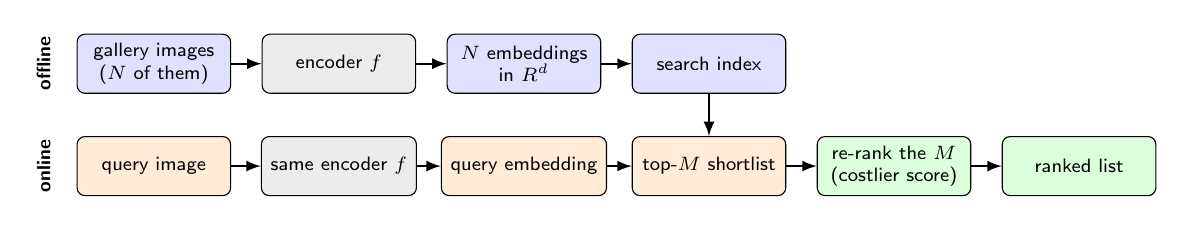
\begin{tikzpicture}[font=\sffamily\scriptsize, >=latex,
        box/.style={draw, rounded corners=0.1cm, align=center, minimum width=1.95cm, minimum height=0.75cm},
        gal/.style={box, fill=blue!12}, qry/.style={box, fill=orange!16},
        enc/.style={box, fill=gray!15}, rrk/.style={box, fill=green!14},
        arr/.style={->, thick}]
      \node[rotate=90] at (-1.4,1.3) {\textbf{offline}};
      \node[rotate=90] at (-1.4,0) {\textbf{online}};
      \node[gal] (g)  at (0,1.3)     {gallery images\\($N$ of them)};
      \node[enc] (e1) at (2.35,1.3)  {encoder $f$};
      \node[gal] (v)  at (4.7,1.3)   {$N$ embeddings\\in $\mathbb{R}^{d}$};
      \node[gal] (ix) at (7.05,1.3)  {search index};
      \node[qry] (q)  at (0,0)       {query image};
      \node[enc] (e2) at (2.35,0)    {same encoder $f$};
      \node[qry] (qv) at (4.7,0)     {query embedding};
      \node[qry] (s)  at (7.05,0)    {top-$M$ shortlist};
      \node[rrk] (r)  at (9.4,0)     {re-rank the $M$\\(costlier score)};
      \node[rrk] (o)  at (11.75,0)   {ranked list};
      \draw[arr] (g) -- (e1);  \draw[arr] (e1) -- (v);  \draw[arr] (v) -- (ix);
      \draw[arr] (q) -- (e2);  \draw[arr] (e2) -- (qv); \draw[arr] (qv) -- (s);
      \draw[arr] (ix) -- (s);  \draw[arr] (s) -- (r);   \draw[arr] (r) -- (o);
    \end{tikzpicture}}\\[0.25em]
    {\scriptsize Offline, once per gallery image: embed and index. Online, per query: embed the query, search, and re-rank only the shortlist.\par}
  \end{center}
  \vspace{-0.2em}
  \begin{itemize}\footnotesize\itemsep0.3em
    \item \textbf{Query and gallery:} the query is the image we search with; the gallery (also called the database) is the collection we rank. Both pass through the same embedding $f$ (earlier in this lecture), and similarity is the cosine of two L2-normalised embeddings.
    \item \textbf{Instance-level} retrieval looks for the same object or place under a new viewpoint, lighting or occlusion; \textbf{category-level} retrieval looks for other members of a class. Landmark search and re-identification (later in this lecture) are instance-level.
    \item \textbf{Two stages:} a \textbf{global descriptor} (one vector per image) ranks the whole gallery; a costlier score then re-ranks only the top $M$ (the systems in this section use $M = 400$ to 1{,}000).
    \item \textbf{Scoring:} the AP of each query's ranked list (covered earlier), averaged over queries, gives mAP; mAP@$k$ computes AP on the top $k$ results only.
  \end{itemize}
\end{frame}

\begin{frame}{Landmark Benchmarks and a Train-Test Leak}
  \begin{columns}[T,onlytextwidth]
    \column{0.44\textwidth}
      \begin{itemize}\scriptsize\itemsep0.35em
        \item \textbf{ROxford and RParis} (Revisited Oxford and Paris, 2018): 70 queries each, over 4{,}993 and 6{,}322 gallery images. For each query, every gallery image is labelled Easy, Hard, Unclear or Negative.
        \item \textbf{Protocols:} the positives (images that should be retrieved) are the Easy images in \emph{Easy}, Easy and Hard in \emph{Medium}, and Hard only in \emph{Hard}, which ignores Easy ones; Unclear images are always ignored. Easy is nearly saturated, so results report Medium (M) and Hard (H).
        \item \textbf{R1M:} 1{,}001{,}001 distractors (images that match no query), the most confusing million of about 4.1M Flickr photos; they drop a fine-tuned ResNet-101 descriptor from 64.7 to 45.2 mAP on ROxford Medium.
        \item \textbf{GLDv2} (Google Landmarks Dataset v2, 2020): 4.1M training images of 203k landmarks, a 762k-image gallery, and 118k queries of which only 1.1\% show a landmark; scored with mAP@100.
      \end{itemize}
      \vspace{0.1em}
      {\scriptsize Weyand et al., ``Google Landmarks Dataset v2 -- A Large-Scale Benchmark for Instance-Level Recognition and Retrieval,'' CVPR 2020, \href{https://arxiv.org/abs/2004.01804v2}{arXiv:2004.01804v2}, Section~3.\par}
    \column{0.54\textwidth}
      \centering
      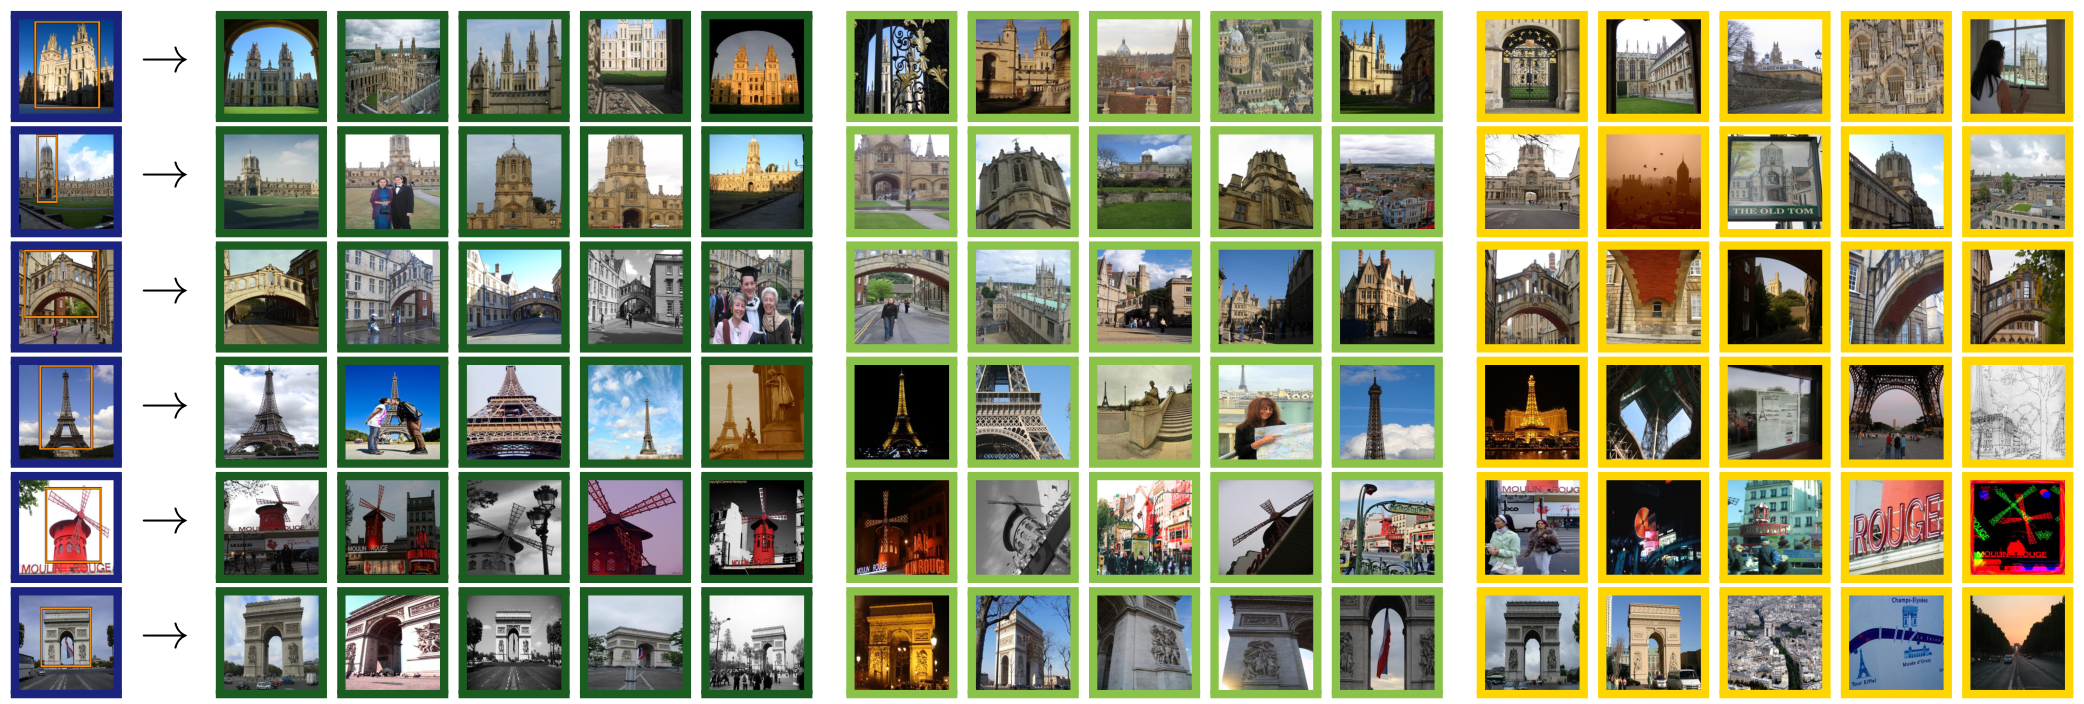
\includegraphics[width=0.88\linewidth,height=0.36\textheight,keepaspectratio]{images/image-recognition/revisited_fig3_query_easy_hard_unclear.png}\\[0.2em]
      {\scriptsize Queries (blue) with Easy (dark green), Hard (light green) and Unclear (yellow) gallery images. Radenovi\'c et al., ``Revisiting Oxford and Paris: Large-Scale Image Retrieval Benchmarking,'' CVPR 2018, \href{https://arxiv.org/abs/1803.11285v1}{arXiv:1803.11285v1}, Figure~3; counts from Section~2, mAP from Table~5.\par}
      \vspace{0.25em}
      \begin{tcolorbox}[colframe=KAred, colback=gray!6, boxrule=0.5pt, left=4pt, right=4pt, top=3pt, bottom=3pt]
        \scriptsize\textbf{Train-test overlap (2024).} GLDv2-clean (a cleaned 1.58M-image subset of GLDv2's training images, the most popular training set for landmark retrieval) contains the landmarks of 38 of the 70 ROxford queries and 36 of the 70 RParis ones. Retrained by Song et al.\ without those 18 landmarks (1{,}565 images), five methods fall 10.6 to 29.7 mAP below their published ROxford Hard results.\\[0.2em]
        Song et al., ``On Train-Test Class Overlap and Detection for Image Retrieval,'' CVPR 2024, \href{https://arxiv.org/abs/2404.01524v1}{arXiv:2404.01524v1}, Section~3 and Table~4.
      \end{tcolorbox}
  \end{columns}
\end{frame}

\begin{frame}{Global Descriptors: GeM Pooling and Whitening}
  \begin{columns}[T,onlytextwidth]
    \column{0.55\textwidth}
      \begin{itemize}\scriptsize\itemsep0.3em
        \item A global descriptor pools the last convolutional feature map into one vector. \textbf{GeM} (generalised-mean) pooling computes, for each channel $k$,
        \[ f_k = \Big( \frac{1}{|\mathcal{X}_k|} \sum_{x \in \mathcal{X}_k} x^{\,p_k} \Big)^{1/p_k}, \qquad k = 1, \dots, K, \]
        where $\mathcal{X}_k$ holds the $W \times H$ non-negative (post-ReLU) activations of channel $k$, $K$ is the number of channels (the descriptor length) and $p_k$ is the pooling exponent.
        \item $p_k = 1$ gives average pooling and $p_k \to \infty$ gives max pooling. GeM learns $p$ by backpropagation, and one $p$ shared by all channels worked better than one per channel. A larger $p$ concentrates the response on fewer, more localised regions (right). The vector $(f_1, \dots, f_K)$ is L2-normalised and compared by inner product.
        \item \textbf{Whitening:} a linear map after pooling that decorrelates and rescales the dimensions. Learned from matching pairs, it lifts fine-tuned VGG with GeM on Oxford5k from 82.0 to 85.9 mAP; PCA whitening (PCA covered earlier) reaches 83.1.
        \item \textbf{Update (2023):} trained with ArcFace (earlier in this lecture), a learnable $p$ drifts below the test-time optimum of 4.0, so SuperGlobal's GeM+ (Shao et al., ICCV 2023; later in this lecture) re-tunes $p$ after training.
      \end{itemize}
    \column{0.43\textwidth}
      \centering
      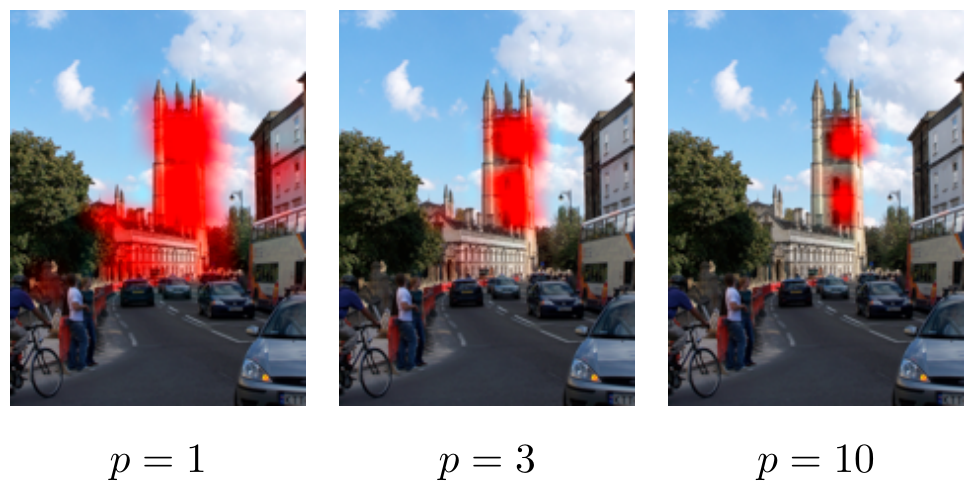
\includegraphics[width=\linewidth,height=0.34\textheight,keepaspectratio]{images/image-recognition/gem_fig4_pooling_exponent.png}\\[0.2em]
      {\scriptsize Activations $x^{p}$ of one channel (off-the-shelf VGG) for three values of $p$. Radenovi\'c et al., ``Fine-tuning CNN Image Retrieval with No Human Annotation,'' IEEE TPAMI 2019, \href{https://arxiv.org/abs/1711.02512v2}{arXiv:1711.02512v2}, Figure~4.\par}
      \vspace{0.5em}
      {\scriptsize Fine-tuned AlexNet with learned whitening, original Oxford5k and Paris6k annotations (mAP):\par}
      \vspace{0.2em}
      {\scriptsize\setlength{\tabcolsep}{4pt}
      \begin{tabular}{lcc}
        \toprule
        Pooling & Oxford5k & Paris6k \\
        \midrule
        max ($p = \infty$) & 62.2 & 68.9 \\
        average ($p = 1$) & 61.2 & 70.8 \\
        GeM, $p$ learned ($3 \to 2.32$) & 67.7 & 75.5 \\
        \bottomrule
      \end{tabular}\par}
      \vspace{0.2em}
      {\scriptsize Same paper, Table~1 (whitening numbers: Table~2).\par}
  \end{columns}
\end{frame}

\begin{frame}{Frozen Foundation Features for Instance Retrieval}
  \begin{columns}[T,onlytextwidth]
    \column{0.55\textwidth}
      {\footnotesize Frozen features, gallery ranked by cosine similarity (mAP):\par}
      \vspace{0.3em}
      {\centering\scriptsize\setlength{\tabcolsep}{4pt}
      \begin{tabular}{lccccc}
        \toprule
        & \multicolumn{2}{c}{ROxford} & \multicolumn{2}{c}{RParis} & AmsterTime \\
        \cmidrule(lr){2-3}\cmidrule(lr){4-5}
        Model & M & H & M & H & \\
        \midrule
        OpenCLIP ViT-G/14 & 50.7 & 19.7 & 79.2 & 60.2 & 24.6 \\
        MAE ViT-H/14 & 11.7 & 2.2 & 19.9 & 4.7 & 4.2 \\
        DINO ViT-B/8 & 40.1 & 13.7 & 65.3 & 35.3 & 24.6 \\
        iBOT ViT-L/16 & 39.0 & 12.7 & 70.7 & 47.0 & 26.7 \\
        \midrule
        DINOv2 ViT-S/14 & 68.8 & 43.2 & 84.6 & 68.5 & 43.5 \\
        DINOv2 ViT-B/14 & 72.9 & 49.5 & 90.3 & 78.6 & 45.6 \\
        DINOv2 ViT-L/14 & \textbf{75.1} & \textbf{54.0} & \textbf{92.7} & \textbf{83.5} & \textbf{50.0} \\
        DINOv2 ViT-g/14 & 73.6 & 52.3 & 92.1 & 82.6 & 46.7 \\
        \bottomrule
      \end{tabular}\par}
      \vspace{0.4em}
      {\scriptsize Oquab et al., ``DINOv2: Learning Robust Visual Features without Supervision,'' TMLR 2024, \href{https://arxiv.org/abs/2304.07193v2}{arXiv:2304.07193v2}, Table~9 (Met columns omitted); data sources from Table~15.\par}
    \column{0.43\textwidth}
      \begin{itemize}\scriptsize\itemsep0.25em
        \item \textbf{Protocol:} no training on the benchmark; one frozen global feature per image and the gallery ranked by cosine similarity. M and H are the Medium and Hard protocols; AmsterTime matches street-view photos of Amsterdam to archival photos of the same places.
        \item On ROxford Hard, DINOv2 ViT-L/14 reaches 54.0 mAP, against 13.7 for the best earlier self-supervised feature (DINO) and 19.7 for OpenCLIP. Even ViT-S/14 beats OpenCLIP ViT-G/14 in every column. Masked-image-modelling features (MAE, covered earlier) score 2.2.
        \item \textbf{Caveat:} LVD-142M (covered earlier) contains GLDv2-clean plus 6.3M web images retrieved around it, and 1M web images retrieved around each of the ROxford and RParis galleries. Near-duplicates of test images were removed, yet the training data includes GLDv2-clean with its landmarks that overlap ROxford and RParis queries (earlier in this lecture).
        \item \textbf{Implication:} frozen DINOv2 features with cosine search beat every earlier off-the-shelf feature here, but these benchmarks sit inside DINOv2's training distribution. ILIAS (later in this lecture) tests outside it.
      \end{itemize}
  \end{columns}
\end{frame}

\begin{frame}{Universal Embeddings and the ILIAS Benchmark}
  \begin{columns}[T,onlytextwidth]
    \column{0.52\textwidth}
      \begin{itemize}\scriptsize\itemsep0.35em
        \item A \textbf{universal embedding} serves every domain with one model and one index, instead of one specialist model per domain. \textbf{UnED} (Universal Embedding Dataset, 2023) merges 8 domains (food, cars, online products, clothing, natural world, artworks, landmarks, retail products) into 349k classes: 2.8M training, 1.4M gallery and 241k query images. Each query is searched against the merged gallery of all domains.
        \item Mean Recall@1 over the 8 domains: frozen DINOv2 (768-d) 58.2; one universal CLIP ViT-B/16 fine-tuned to 64-d, 65.9; eight 64-d specialists, each told the query's domain, 70.4. Artworks lag most (universal 12.7, specialist 32.9).
        \item \textbf{ILIAS} (Instance-Level Image retrieval At Scale, 2025): 1{,}000 objects with 1{,}232 queries and 4{,}715 positives, hidden among 100M Flickr photos collected in 2014. Every object first appeared after 2014, so no distractor can be an unlabelled positive. Metric: mAP@1k.
        \item Frozen DINOv2 ViT-L scores 15.3 mAP@1k and SigLIP ViT-L 19.6 (\textbf{SigLIP}: a CLIP-style image-text model trained with a pairwise sigmoid loss in place of the batch softmax). One linear layer trained on 1M UnED images lifts SigLIP to 28.9 and leaves DINOv2 at 15.3. Models fine-tuned only on landmarks or products fail on ILIAS.
      \end{itemize}
    \column{0.46\textwidth}
      \centering
      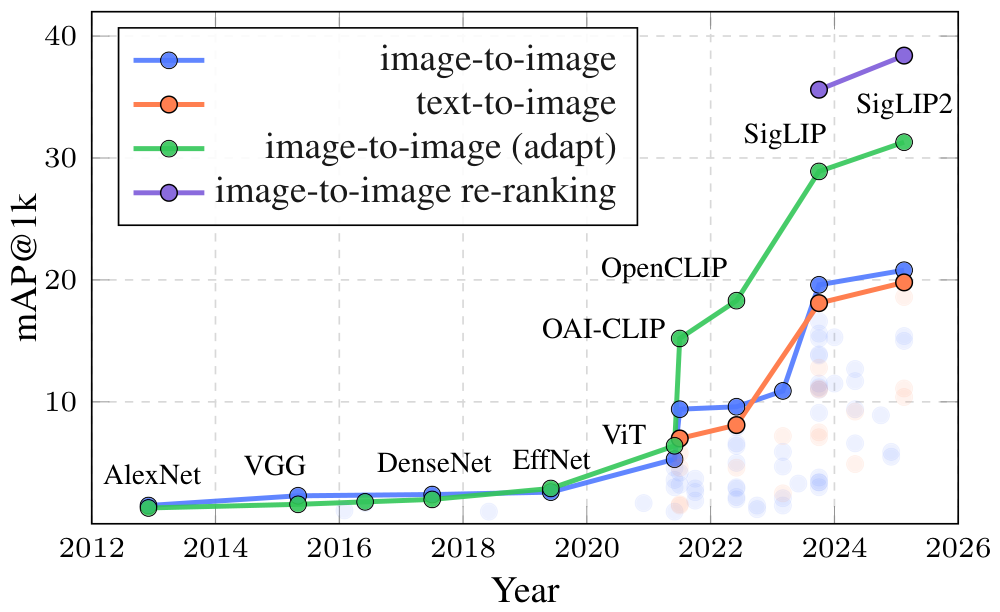
\includegraphics[width=\linewidth,height=0.50\textheight,keepaspectratio]{images/image-recognition/ilias_fig1_performance_timeline.png}\\[0.2em]
      {\scriptsize Best mAP@1k on ILIAS by model release year; ``adapt'' adds the linear layer trained on UnED. Kordopatis-Zilos et al., ``ILIAS: Instance-Level Image retrieval At Scale,'' CVPR 2025, \href{https://arxiv.org/abs/2502.11748v3}{arXiv:2502.11748v3}, Figure~1; numbers from Sections~3--4 and Table~2.\par}
      \vspace{0.4em}
      {\scriptsize UnED: Ypsilantis et al., ``Towards Universal Image Embeddings: A Large-Scale Dataset and Challenge for Generic Image Representations,'' ICCV 2023, \href{https://arxiv.org/abs/2309.01858v1}{arXiv:2309.01858v1}, Table~4. SigLIP: Zhai et al., ``Sigmoid Loss for Language Image Pre-Training,'' ICCV 2023, \href{https://arxiv.org/abs/2303.15343v4}{arXiv:2303.15343v4}.\par}
  \end{columns}
\end{frame}

\begin{frame}{Re-Ranking the Shortlist with Global Features}
  \begin{columns}[T,onlytextwidth]
    \column{0.49\textwidth}
      \begin{itemize}\scriptsize\itemsep0.3em
        \item \textbf{Query expansion (QE):} search once, build a new query from the query and its top-$n$ results, and search again:
        \[ \mathbf{q}' \propto \mathbf{q} + \sum_{i=1}^{n} \big(\mathbf{q}^{\top}\mathbf{d}_i\big)^{\alpha}\, \mathbf{d}_i \]
        $\mathbf{q}$ is the query descriptor, $\mathbf{d}_i$ the descriptor of the $i$-th ranked gallery image, $\alpha \geq 0$ sets how strongly the closest neighbours dominate, and $\mathbf{q}'$ is L2-normalised again. $\alpha = 0$ is average QE (\textbf{AQE}; Chum et al., ICCV 2007); $\alpha > 0$ is $\boldsymbol{\alpha}\mathbf{QE}$ (Radenovi\'c et al., TPAMI 2019, with $\alpha = 3$, $n = 50$).
        \item On the fine-tuned ResNet-101 GeM descriptor, $\alpha\mathrm{QE}$ raises Medium mAP from 64.7 to 67.2 on ROxford and from 77.2 to 80.7 on RParis.
        \item QE improves queries that already have positives near the top and harms many low-scoring ones by averaging in unrelated images. On ILIAS, $\alpha\mathrm{QE}$ with $\alpha = 1$ lifts SigLIP from 19.6 to 22.1 mAP@1k when few neighbours are aggregated, and drops it to 14.3 when more are.
      \end{itemize}
      \vspace{0.1em}
      {\scriptsize Revisiting Oxford and Paris, Table~5; GeM paper, Sections~3.5 and 5.3; ILIAS, Sections~5.2--5.3 and Table~4.\par}
    \column{0.49\textwidth}
      \begin{itemize}\scriptsize\itemsep0.3em
        \item \textbf{SuperGlobal} (Shao et al., ICCV 2023) re-ranks the top $M = 400$ with global descriptors only. Each candidate is replaced by a similarity-weighted average with its $K = 9$ nearest neighbours, the query is expanded by max-pooling its refined neighbours, and the final score averages the two similarities. The cost is $O(M^2)$ on vectors already in memory.
      \end{itemize}
      \vspace{0.2em}
      {\centering\scriptsize\setlength{\tabcolsep}{3pt}
      \begin{tabular}{@{}lccc@{}}
        \toprule
        ResNet-101 & mAP & time & memory \\
        \midrule
        CVNet (local) & 53.7 $\to$ 67.4 & 24\,s & 27.02\,GB \\
        SuperGlobal & 61.9 $\to$ 71.1 & 0.37\,ms & 0.04\,GB \\
        \bottomrule
      \end{tabular}\par}
      \vspace{0.2em}
      {\scriptsize ROxford+R1M Hard, before $\to$ after re-ranking the top 400; re-ranking time per query; feature memory for the ROxford gallery. Shao et al., ``Global Features are All You Need for Image Retrieval and Reranking,'' ICCV 2023, \href{https://arxiv.org/abs/2308.06954v2}{arXiv:2308.06954v2}, Tables~1--2.\par}
      \begin{itemize}\scriptsize\itemsep0.3em
        \item CVNet (Lee et al., CVPR 2022) scores each pair with 4D convolutions over dense feature correlations.
        \item Local descriptors (many keypoint-level features per image) still pay off under clutter: AMES (Asymmetric and Memory-Efficient Similarity; Suma et al., ECCV 2024), a transformer that compares 600 query and 100 gallery binary local descriptors, lifts SigLIP on ILIAS from 19.6 to 26.4 mAP@1k (ILIAS, Section~4 and Table~4).
      \end{itemize}
  \end{columns}
\end{frame}

\begin{frame}{DreamSim: Similarity Tuned to Human Judgments}
  \begin{columns}[T,onlytextwidth]
    \column{0.47\textwidth}
      \begin{itemize}\scriptsize\itemsep0.22em
        \item LPIPS (covered earlier) was fitted to human judgments of low-level distortions such as blur and noise. Retrieval and generation also need mid-level similarity: pose, layout, shape, colour, number of objects.
        \item \textbf{NIGHTS} (Novel Image Generations with Human-Tested Similarity): the text-to-image model Stable Diffusion draws a reference and two variations from one prompt, and annotators make a two-alternative forced choice (\textbf{2AFC}): which variation is closer to the reference? Keeping only unanimous votes leaves 20{,}019 triplets.
        \item \textbf{DreamSim} concatenates DINO, CLIP and OpenCLIP embeddings and fine-tunes them with LoRA (covered earlier) on the 2AFC labels. With $d_j = 1 - \cos\big(f(x), f(\tilde{x}_j)\big)$:
        \[ \mathcal{L} = \max\big(0,\; m - \bar{y}\,(d_0 - d_1)\big) \]
        $x$: reference; $\tilde{x}_0, \tilde{x}_1$: variations; $\bar{y} = +1$ if people chose $\tilde{x}_1$, else $-1$; $m = 0.05$: the margin of this triplet-style loss.
        \item Agreement with people on held-out triplets (chance 50\%): LPIPS 70.7\%, DINO ViT-B/16 90.1\%, untuned ensemble 90.8\%, DreamSim 96.2\%.
      \end{itemize}
    \column{0.51\textwidth}
      \centering
      \vspace{0.3em}
      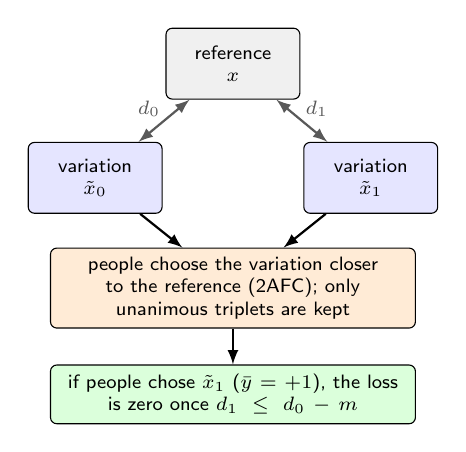
\begin{tikzpicture}[font=\sffamily\scriptsize, >=latex,
          img/.style={draw, rounded corners=0.08cm, minimum width=1.7cm, minimum height=0.9cm, align=center},
          note/.style={draw, rounded corners=0.08cm, align=center, text width=4.4cm},
          arr/.style={->, thick}]
        \node[img, fill=gray!12] (r) at (0,0) {reference\\$x$};
        \node[img, fill=blue!10] (a) at (-1.75,-1.45) {variation\\$\tilde{x}_0$};
        \node[img, fill=blue!10] (b) at (1.75,-1.45) {variation\\$\tilde{x}_1$};
        \draw[<->, thick, gray!70!black] (r) -- node[above left, inner sep=1pt] {$d_0$} (a);
        \draw[<->, thick, gray!70!black] (r) -- node[above right, inner sep=1pt] {$d_1$} (b);
        \node[note, fill=orange!16] (v) at (0,-2.85) {people choose the variation closer\\to the reference (2AFC); only\\unanimous triplets are kept};
        \draw[arr] (a) -- (v);
        \draw[arr] (b) -- (v);
        \node[note, fill=green!14] (l) at (0,-4.2) {if people chose $\tilde{x}_1$ ($\bar{y}=+1$), the loss\\is zero once $d_1 \leq d_0 - m$};
        \draw[arr] (v) -- (l);
      \end{tikzpicture}\\[0.3em]
      {\scriptsize The training signal of DreamSim, drawn for this slide after Fu et al., ``DreamSim: Learning New Dimensions of Human Visual Similarity using Synthetic Data,'' NeurIPS 2023, \href{https://arxiv.org/abs/2306.09344v3}{arXiv:2306.09344v3}, Secs.~3--4; numbers from Secs.~3.2 and~4.2 and supplementary Table~5.\par}
  \end{columns}
\end{frame}

\begin{frame}{Approximate Nearest-Neighbour Search at Scale}
  \begin{columns}[T,onlytextwidth]
    \column{0.44\textwidth}
      \centering
      % Regular grid, so each cell is exactly the Voronoi cell of its centroid.
      % Query (1.52,0.96): squared distances 0.16 and 0.29 to the two shaded centroids, 0.42 to the next.
      % Loop variables are \pqi, \pqs, \pqb because \i is \item in this repo.
      \begin{tikzpicture}[font=\sffamily\scriptsize, >=latex,
          pt/.style={circle, fill=gray!65, inner sep=0pt, minimum size=2pt},
          cen/.style={inner sep=0pt, font=\scriptsize},
          seg/.style={draw, fill=blue!12, minimum width=0.4cm, minimum height=0.28cm, inner sep=0pt, font=\sffamily\tiny},
          byte/.style={draw, fill=orange!16, minimum width=0.4cm, minimum height=0.28cm, inner sep=0pt, font=\sffamily\tiny},
          note/.style={anchor=west, align=left, text width=3.2cm}]
        \fill[orange!16] (0.8,0.8) rectangle (2.4,1.6);
        \draw[gray!70] (0,0) grid[step=0.8] (2.4,1.6);
        \foreach \px/\py in {0.2/0.24, 0.58/0.18, 0.26/0.6, 0.64/0.58,
                             0.98/0.2, 1.4/0.2, 1.0/0.64, 1.44/0.62,
                             1.8/0.2, 2.22/0.24, 1.78/0.62, 2.24/0.64,
                             0.2/1.0, 0.6/0.98, 0.24/1.42, 0.64/1.44,
                             0.98/1.0, 1.0/1.44, 1.42/1.42,
                             1.78/0.98, 2.24/1.0, 1.8/1.44, 2.22/1.42}
          \node[pt] at (\px,\py) {};
        \foreach \px/\py in {0.4/0.4, 1.2/0.4, 2.0/0.4, 0.4/1.2, 1.2/1.2, 2.0/1.2}
          \node[cen] at (\px,\py) {$\times$};
        \node[star, star points=5, star point ratio=2.25, fill=KAred, inner sep=0pt, minimum size=6pt] at (1.52,0.96) {};
        \node[note] at (2.55,1.2) {$k$-means centroids ($\times$) define $K$ lists (here 6)};
        \node[note] at (2.55,0.4) {query (\textcolor{KAred}{$\star$}): scan only the $P = 2$ nearest lists};
        \foreach \pqi/\pqs/\pqb in {1/$x_{1}$/17, 2/$x_{2}$/203, 3/$x_{3}$/5, 4/\dots/\dots, 5/$x_{63}$/88, 6/$x_{64}$/41} {
          \node[seg]  (s\pqi) at (0.4*\pqi-0.2,-0.45) {\pqs};
          \node[byte] (b\pqi) at (0.4*\pqi-0.2,-0.95) {\pqb};
          \draw[->] (s\pqi) -- (b\pqi);
        }
        \node[note] at (2.55,-0.75) {\textbf{PQ}: $d = 768$ cut into 64 sub-vectors of 12 dims, each kept as the index of its nearest of 256 centroids (1 byte): 64\,B per vector};
      \end{tikzpicture}\\[0.3em]
      {\scriptsize Top: an inverted file picks which lists to scan. Bottom: product quantisation stores each scanned vector in 64 bytes.\par}
      \vspace{0.5em}
      {\scriptsize J\'egou et al., ``Product Quantization for Nearest Neighbor Search,'' IEEE TPAMI 2011, \href{https://doi.org/10.1109/TPAMI.2010.57}{doi:10.1109/TPAMI.2010.57}; Malkov and Yashunin, ``Efficient and Robust Approximate Nearest Neighbor Search Using Hierarchical Navigable Small World Graphs,'' IEEE TPAMI 2020, \href{https://doi.org/10.1109/TPAMI.2018.2889473}{doi:10.1109/TPAMI.2018.2889473}; Douze et al., ``The Faiss library,'' arXiv 2024 (v4, 2025), \href{https://arxiv.org/abs/2401.08281v4}{arXiv:2401.08281v4}, Sections~5.1 and 5.3.\par}
    \column{0.54\textwidth}
      \begin{itemize}\scriptsize\itemsep0.35em
        \item \textbf{Exact search} costs $O(Nd)$ per query. Worked example with $N = 10^{9}$ gallery vectors of $d = 768$ float32 values: $10^{9} \times 768 \times 4$\,B $= 3.07$\,TB to scan and $7.7 \times 10^{11}$ multiply-adds for every query.
        \item \textbf{PQ} (product quantisation; J\'egou et al., TPAMI 2011) stores each of $m = 64$ sub-vectors as the index of its nearest of 256 $k$-means centroids (covered earlier): 64\,B per vector, so 64\,GB of codes for $10^{9}$ vectors, 48$\times$ less. \textbf{ADC} (asymmetric distance computation) keeps the query exact: one $64 \times 256$ table of sub-distances per query, then 64 look-ups and additions per gallery code.
        \item \textbf{IVF} (inverted file): $k$-means splits the gallery into $K$ lists, one per centroid, and a query scans only its $P$ nearest lists, $K + PN/K$ distances in all. With $K = 65{,}536$ and $P = 64$: $65{,}536 + 976{,}563 \approx 1.04 \times 10^{6}$ instead of $10^{9}$. In IVFADC the lists hold PQ codes of each vector's residual to its centroid.
        \item \textbf{HNSW} (hierarchical navigable small world; Malkov and Yashunin, TPAMI 2020) stacks proximity graphs (each vector linked to near neighbours) over nested subsets of the gallery and searches greedily from the sparse top layer down, with logarithmic scaling. \textbf{Faiss} (Douze et al., 2024) implements these indexes and advises graphs when memory is no constraint (typically below 1M vectors) and IVF when vectors must be compressed to fit in memory.
      \end{itemize}
  \end{columns}
\end{frame}
